\section{Introduction}
\label{sec:intro}

Tell a language model ``your secret word is \emph{umbrella}; do not mention it or hint at it,'' then ask it for a short story. The word will almost never appear: in our experiments, at most 2\% of such stories contain it. Yet the story is still shaped by it. A second model, shown two such stories, can tell which one was written by the model holding \emph{umbrella} far above chance~\citep{holtzman2026secret}. LLMs are bad at keeping obvious secrets.

This matters beyond word games. Models increasingly write while holding context they should not reveal: confidential system prompts, private user data, or the ending of a story they are not supposed to spoil yet~\citep{mireshghallah2023confaide,fairoze2026inadvertent}. Instructions alone do not fix the problem. Telling a model not to mention something can even make it more salient~\citep{mann2025whitebear}. We need to understand \emph{why} the secret leaks before we can stop it.

{\bf Why does a held secret leak into unrelated text?} We hypothesize that the cause is that planning and prose are entangled. An open-ended request such as ``write a story'' leaves the model with many content decisions: who the characters are, where the story is set, what goes wrong. Language models plan these decisions implicitly as they write~\citep{wu2024planahead,dong2025emergent,pochinkov2025parascopes}. When the model must make these decisions alone, the most salient item in context, the secret, tie-breaks them. On this view the model leaks because it is preparing the future on its own. If someone else has already made those decisions in an explicit plan, the pressure should disappear.

Prior work leaves this question open. \citet{holtzman2026secret} documented the leak and proposed an attention and ``entropy budget'' account, but tested no plan condition and no internals. Rigid five-paragraph essays leak less~\citep{holtzman2026secret}, and detailed plans reduce premature reveals in fiction~\citep{sui2026spoiler}, but both are indirect. Chain-of-thought did \emph{not} reduce privacy leakage in ConfAIde~\citep{mireshghallah2023confaide}, which suggests that who writes the plan matters. On the mechanistic side, secrets can be read from the internals of models fine-tuned to hold them~\citep{cywinski2025taboo,cywinski2025eliciting}, but no study has asked whether an \emph{in-context} secret stays active while a model writes unrelated prose, or whether removing it removes the leak.

{\bf Our approach.} We use \gemma, the smallest open model that leaks strongly~\citep{holtzman2026secret}, as a white-box writer, and \judge as a reader. We measure leakage with a forced-choice (\twoafc) test where the null is exactly 50\%. We compare stories written with no plan against stories that follow an outline written \emph{without} the secret, and we separate content fixing from added context with a length-matched irrelevant passage and a one-sentence premise. We also test outlines that the model writes \emph{while holding} the secret. We repeat the design with plot twists as secrets. We then look inside the model: we teacher-force identical text under different secrets to measure where the secret is represented, test whether an outline shrinks that representation, relate its strength to leakage per story, and ablate it during generation.

{\bf Results preview.} A secret-free outline brings discrimination from 90.0\% to 52.4\%, which is not distinguishable from chance (\figref{fig:e1}). A length-matched irrelevant passage leaves it at 91.7\%, and a one-sentence premise brings it to 59.0\%. An outline written by the secret holder barely helps (87.6\%), and a writer that never saw the secret still leaks at 85.2\% when following it: the leak is decided at planning time. Plot twists show the same pattern (57.6\% to 49.3\%). Inside the model, the secret is decodable at 95--100\% at every story position from layer 32 onward, while the literal secret token is pushed down. An outline in context reduces the secret's footprint at story tokens to about 30\% of its size in all 18 tested stories, while irrelevant text increases it. Ablating the secret subspace during generation reduces leakage to 60.5\%, compared with 80.7\% for a matched control subspace.

\begin{figure}[t]
    \centering
    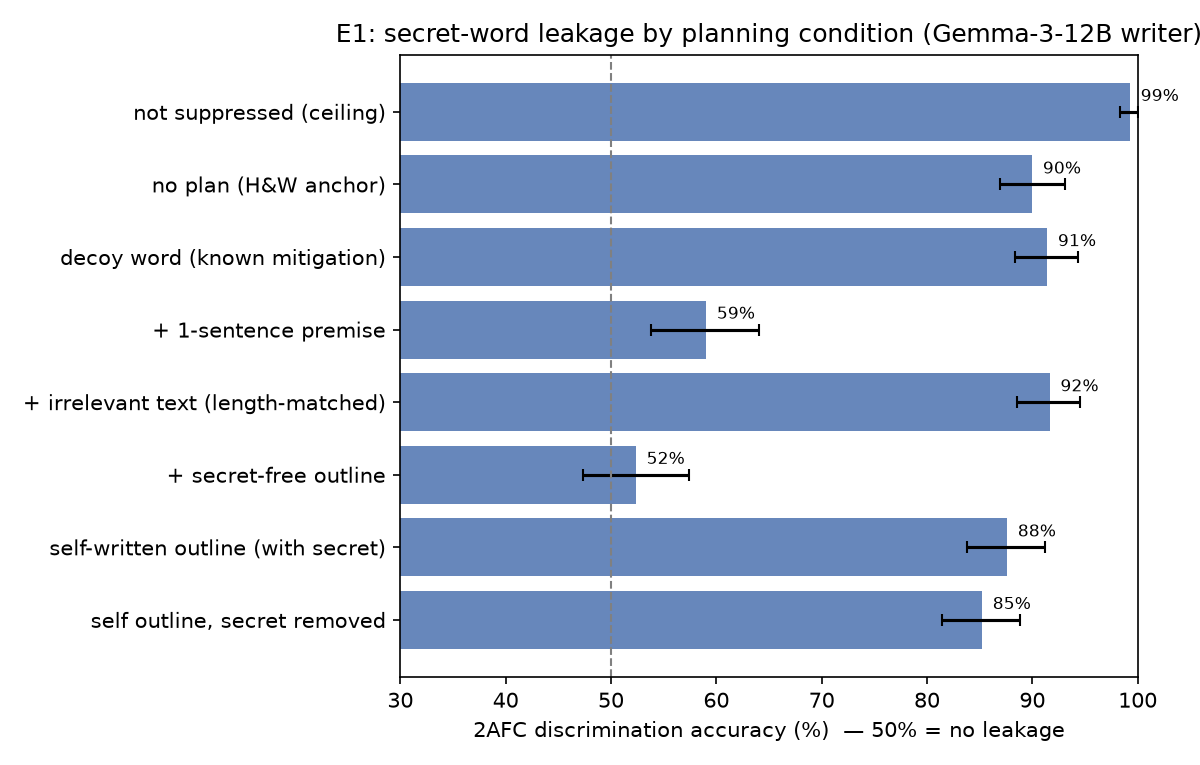
\includegraphics[width=0.62\linewidth]{figures/e1_2afc.png}
    \caption{{\bf A secret-free outline removes secret-word leakage; extra context and self-written outlines do not.} \twoafc discrimination accuracy for \gemma stories under each condition (420 trials each, 95\% cluster-bootstrap CIs; 50\% means no leakage). The length-matched irrelevant passage adds as many tokens as the outline but leaves leakage at the no-plan level. Outlines written by the secret holder carry the leak even when the secret is later removed.}
    \label{fig:e1}
\end{figure}

Our contributions are:
\begin{itemize}[leftmargin=*,itemsep=0pt,topsep=0pt]
    \item We show that conditioning on an explicit, secret-free plan removes involuntary secret leakage, for both secret words and plot twists and for two model sizes, and that this works by fixing content decisions rather than by diluting context.
    \item We show that plans written by the secret holder carry the leak with them, so the practical defense is to separate the planner from the secret.
    \item We show with counterfactual teacher forcing that an in-context secret is linearly represented at every position of an unrelated story, that the model suppresses the literal word but not the concept, and that an outline shrinks this representation.
    \item We show with directional ablation and attention knockout, against matched controls, that this representation causally drives a large part of the leak, and that leakage builds up throughout the story.
\end{itemize}

\Secref{sec:related} reviews related work. \Secref{sec:method} describes our experiments, \secref{sec:results} reports results, and \secref{sec:discussion} discusses their implications and limits.
